\documentclass[]{article}
\usepackage{listings}
\usepackage{hyperref}
\usepackage{graphicx}

%Commands
\newcommand{\kb}{kulturBOT}
\newcommand{\kbspace}{\kb \space}
\newcommand{\mykb}{my \kb}
\newcommand{\mykbspace}{\mykb \space}

%Code Styles
\lstdefinestyle{ssh}{
	showspaces=true,
	frame=single
}

% Title Page
\title{\kbspace Instruction Manual}
\author{Colin Gagich \\ \textnormal Version 2.0}
\date{Last Updated: \today}

\begin{document}
\maketitle

\newpage

\tableofcontents
\newpage

\section{Getting Started}
Hello there! You have been tasked with taking care of \mykb! Welcome to the team! We are glad to have you with us. Here are some things to get you started working with \kb.

\subsection{Quick Facts}

Twitter Profile: \href{https://twitter.com/kulturBOT}{@kulturBOT} \\
Facebook Profile: \href{https://www.facebook.com/thekulturbot}{Facebook Homepage}\\
Expected Battery Life: 3 Hours.\\
Expected Charge Time: 3 Hours.\\ \\
\textbf{DO NOT LIFT \kbspace BY THE HANDLES OF THE STRAINER} - Instead lift the robot from the white base.

\subsection{\mykb 's Anatomy}

\mykbspace is made from a version of the iRobot Create which is directly related to the popular in house robotic vacuum cleaner. Hidden under the front of the strainer, \kbspace has three buttons. These three buttons are used to control various functions of \kb. Refer to Figure \ref{3button} for the names of these buttons. Also take note of the names of the LED's.

	\begin{figure}[h!]
		\centering
	    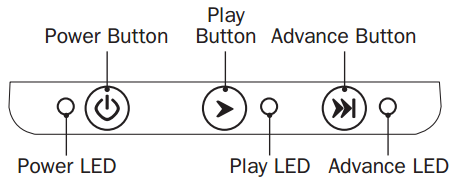
\includegraphics[width=0.8\textwidth]{img/3button.png}
	    \caption{Three Buttons Found Under Strainer}
	    \label{3button}
	\end{figure}

\subsection{Turning \kbspace on.}
\begin{enumerate}
\item Press the \texttt{Power Button}. The \texttt{Power LED} should now be green and you will hear a \textit{beep}.
\item The main white Dome light will also turn on when \kbspace is on.
\end{enumerate}

\subsubsection{Is \kbspace turned on?}
\label{isKbOn}
To determine if \kbspace is on, observe the \texttt{Power LED}. If it is \texttt{Green}, \kbspace is on. If it is \texttt{Orange/Amber} \kbspace is on but needs to be charged (See Section \ref{chargingKB}). If the \texttt{Power LED} is not on, \kbspace is either off or the batteries are dead.\\
The main Dome light will also be on when \kbspace is on.

\subsubsection{Restarting \kb}
\label{restartKb}
From time to time you will need to restart \kbspace. To restart \kb:

\begin{enumerate}
\item Press the \texttt{Power Button}. The \texttt{Power LED} should now be off.
\item Press the \texttt{Power Button} again. The \texttt{Power LED} should now be green and you will hear a \textit{beep}.
\item After around 20 seconds \kbspace will start moving.
\end{enumerate}

\subsection{Virtual Walls}
Use the virtual walls to prevent \kbspace from leaving a room or getting too close to delicate items. To turn them on press the power button on the front so the green LED is illuminated.\\

\textbf{NOTE: } The walls will only stay on for 45 minutes at a time and must be turned on again when the LED turns off.

\section{Normal Operation}
The following outlines how to get \mykbspace operating normally.


\subsection{Using the \mykbspace Unit}
\label{connect2kb}
First ensure \kbspace is turned on. Refer to \ref{isKbOn}.

\begin{enumerate}
	\item The main dome light should be on - it is a bright white LED array (which is very hard to miss).
	\item There is a small green LED on the printer which should be blinking once every 2 seconds. This indicates the printer is functioning properly.
	\item The unit will then operate on its own - repeating a stop - go - stop -print cycle until it is powered down or its batteries have died.
\end{enumerate}

\subsection{Stopping \mykb}
\label{stoppingKb}
\begin{enumerate}
\item Wait until \kbspace has temporarily stopped moving. This should happen every 45-60 seconds. It is best to turn \kbspace off just after a poem has printed. Press the power button once to turn off \kb. The main dome light should be off.
\item It is important \mykbspace \textbf{is not turned off shortly after being turned on.} This may cause corruption of the onboard memory - before turning it off wait until \kbspace has moved.

\end{enumerate}

%If you were unable to stop \kbspace using the previous steps, try these next:

%\begin{enumerate}
%\item Find the \kbspace unit.
%\item \textit{Aggressively} press the \texttt{Power Button} as depicted in Figure \ref{3button}.
%\end{enumerate}

\subsection{Charging \mykb}
\label{chargingKB}

\begin{enumerate}
\item Determine if the \kbspace unit is on. Refer to Section \ref{isKbOn}
\item IF \kbspace \textbf{is on}, stop it if it is running (See Section \ref{stoppingKb}).
\item Plug \kbspace into the provided wall adapter. The chargingout outlet on \kbspace is on the right rear side section.
\item The main dome will light up and about 10 seconds after it is plugged in the Red Printer Status light will fade slowly indicating it is charging. Note: \textbf{The red light will still fade on and off even when \kbspace is fully charged.}
\end{enumerate}

\section{Normal Behaviour}

This section will describe the "loop" which \kbspace follows. If \kbspace is behaving in any other way, it should be stopped and restarted.

\begin{enumerate}
\item After turning on, \kbspace will \textit{beep} and start moving.
\item After 45 seconds, \kbspace will stop. The robot may play a song if it deems it necessary.
\item After 90 seconds, \kbspace will \textit{beep} and start moving again.
\item This cycle will repeat a few times until \kbspace comes to a stop and the Red Light Bar by the printer starts flashing.
\item A poem will then print and the light bar will continue to flash for 20 seconds allowing adequate time for the print to be collected by a bystander.
\end{enumerate}

The robot will then reboot and repeat the cycle.
\\

When \kbspace is stopped, it will do one of three things:

\begin{enumerate}
\item Make loud robot noises.
\item Print a poem.
\item Do nothing.
\end{enumerate}

After 3 hours \kbspace should be charged. See Section \ref{chargingKB}.

\section{Maintenance}
\subsection{Replacing the paper}
If you noticed a purple/pink streak in the prints - the paper is low and should be replaced soon. Note: The paper can be feed line by line by pressing the small black button on the top of the printer.
\begin{enumerate}
\item Ensure \mykbspace is \textbf{off}.
\item Open the printer by pulling up the small tab.
	\begin{figure}[h!]
		\centering
	    \includegraphics[width=0.8\textwidth]{img/tab.jpg}
	    \caption{Opening printer paper compartment}

	\end{figure}
\item Remove the remaining paper spool.
\item Open a new paper spool and remove the first layer.
\item Place the spool such that \textbf{LOOSE END ON THE BOTTOM OF THE SPOOL.} Ensure there is an excess length of paper on the bottom of the spool.
	\begin{figure}[h!]
		\centering
	    \includegraphics[width=0.8\textwidth]{img/paper.jpg}
	    \caption{Placing spool in compartment}

	\end{figure}
\item Press the printer cover down firmly. The tab will move back into place on its own.
	\begin{figure}[h!]
		\centering
	    \includegraphics[width=0.8\textwidth]{img/close.jpg}
	    \caption{Closing paper compartment}
	\end{figure}
\item Rip off the extra length of paper. This leaves a clean edge for the next print.
\end{enumerate}
\subsection{Preparing for shipping}

Remove the flag by firmly pulling it upwards about 2 inches. Then point the flag horizontally and pull it out.\\ 

	\begin{figure}[h!]
		\centering
	    \includegraphics[width=0.8\textwidth]{img/out.jpg}
	    \caption{Flag Pole - Horizontal}
	\end{figure}
	
\newpage

The flag can be broken down into two pieces (in a camping pole like fashion) for shipping.

	\begin{figure}[h!]
		\centering
	    \includegraphics[width=0.8\textwidth]{img/camp.jpg}
	    \caption{Flag Pole}
	\end{figure}
\newpage
\section{Troubleshooting}
\subsection{\kbspace is moving but no longer stopping!}
Try to catch the robot and lift it up by the base. \textbf{DO NOT LIFT \kbspace BY THE HANDLES OF THE STRAINER} This will cause to the robot to stop moving.
\subsection{\kbspace printed an error message!}
Uh oh! The on board memory may need to be replaced!!!
\subsection{\kbspace won't turn on.}
\kbspace batteries are probably dead. See the instructions in Section \ref{chargingKB}.
\subsection{\kbspace has become self aware!}
Well .. I'll take your word for it; but it is now your problem!
\subsection{Something else has happened!}
Try restarting \underline{everything}. Laptop, \kb, and anything else. If you are still having issues contact \texttt{Colin Gagich - colin.gagich@gmail.com}
\end{document}          
